% Chapter 6: Is the iPhone suitable as a robot's sensor and compute platform? First draft.
% Sources: literature in references.bib (phone-as-robot block, added 2026-10-27);
%   motion-capture sessions Oct 26-27, 2026 (/mnt/project-files/velocity-experiment/,
%   analyze_velocity.py pass criteria P1-P9); Terra PR #89 sensor timing probe and
%   tools/sensor_timing/ (first capture 2026-10-27 18:37Z, iPhone17,2, iOS 27.0.1, Debug);
%   Zorvane bucket-detector evaluation 2026-10-27 (/mnt/project-files/bucket-detector-sim/);
%   Terra code: ObjectSearchDetector.swift, SensorTimingProbe.swift, PhoneController.swift.
% Every number in a "measured" cell comes from one of those sources. Cells marked
% "pending" have a protocol below and no data yet. Do not fill them by estimate.

\DeclareRobustCommand{\evfull}{\tikz[baseline=-0.6ex]\fill (0,0) circle (0.7ex);}
\DeclareRobustCommand{\evhalf}{\tikz[baseline=-0.6ex]{\draw (0,0) circle (0.7ex); \fill (0,-0.7ex) arc (-90:90:0.7ex) -- cycle;}}
\DeclareRobustCommand{\evnone}{\tikz[baseline=-0.6ex]\draw (0,0) circle (0.7ex);}

\chapter{Is a Phone Enough? The iPhone as Sensor Head and Computer}
\label{ch:phone}

The whole design of this thesis rests on one claim: a single consumer phone can be the rover's only sensor head and its only computer.
Chapters~\ref{ch:rover} and~\ref{ch:autonomy} assumed this and built on it.
This chapter tests it.

The question is not whether a phone \emph{can} drive a robot; earlier work shows it can (Section~\ref{sec:phone-lit}).
The question is whether the phone meets the specific numbers that Terra's control loop, map, detector and outdoor guidance depend on, under the load of all of them running at once, on a moving ground vehicle, for the length of a match.
The chapter first turns the rest of the thesis into measurable requirements, then reviews what the literature already establishes for each, names what it leaves open, and fills those gaps with experiments on the rover.
Some of those experiments are complete, some have partial data, and some are designed but not yet run.
Their status is marked in every table, and no pending cell contains an estimate.

\section{Platform under test}
\label{sec:phone-platform}

All measurements in this chapter use the phone mounted on CrabTrapBot (Chapter~\ref{ch:rover}): an iPhone Pro with a LiDAR scanner, hardware identifier iPhone17,2 (iPhone~16 Pro Max), running iOS~27.0.1.
Figure~\ref{fig:phone-pipeline} shows which phone subsystems Terra uses and where each sample is timestamped on its way to the motors.

\begin{figure}[ht]
\centering
\begin{tikzpicture}[
  box/.style={draw, rounded corners=2pt, align=center, font=\footnotesize, inner sep=3pt},
  arr/.style={-{Latex[length=2mm]}, thick},
  stamp/.style={font=\scriptsize, inner sep=1pt}
]
% sensors column
\node[box, text width=3.0cm, minimum height=0.9cm] (imu) at (0, 3.3) {IMU\\Core Motion, 100~Hz};
\node[box, text width=3.0cm, minimum height=0.9cm] (cam) at (0, 1.8) {Camera + LiDAR\\ARKit VIO, depth};
\node[box, text width=3.0cm, minimum height=0.9cm] (gps) at (0, 0.3) {GNSS + compass\\Core Location};
\node[box, text width=3.0cm, minimum height=0.9cm] (npu) at (0,-1.2) {Neural Engine\\Core ML, YOLO};
% swift and rust
\node[box, text width=2.6cm, minimum height=5.4cm] (swift) at (4.7, 1.05) {\textbf{TerraPhone}\\(Swift)\\[4pt] sensor handlers\\[4pt] serial\\\texttt{terra.control}\\queue\\[4pt] depth $\to$\\occupancy grid};
\node[box, text width=2.6cm, minimum height=5.4cm] (rust) at (8.5, 1.05) {\textbf{Terra core}\\(Rust)\\[4pt] estimator\\[2pt] planner\\[2pt] speed loop\\100~Hz\\[2pt] safety gates};
\node[box, text width=1.8cm, minimum height=0.9cm] (pi) at (11.9, 1.05) {Pi bridge\\$\to$ motors};
\foreach \s in {imu,cam,gps,npu} \draw[arr] (\s.east) -- (\s.east -| swift.west);
\draw[arr] (swift.east) -- (rust.west);
\draw[arr] (rust.east) -- node[above, font=\scriptsize]{BLE} node[below, font=\scriptsize]{20~Hz} (pi.west);
% timestamps
\node[stamp, above=1pt] at (imu.north) {$t_{\text{sensor}}$};
\node[stamp, above] at ($(imu.east)!0.5!(imu.east -| swift.west)$) {$t_{\text{os}}$};
\node[stamp, above=1pt] at (swift.north) {$t_{\text{queue}}$};
\node[stamp, above] at ($(swift.east)!0.5!(rust.west)$) {$t_{\text{done}}$};
\end{tikzpicture}
\caption{The phone's role on Terra. Each IMU, AR, detector and GPS sample is stamped when the sensor produced it ($t_{\text{sensor}}$), when iOS handed it to the app ($t_{\text{os}}$), when its block started on the control queue ($t_{\text{queue}}$), and when it reached Rust ($t_{\text{done}}$) (Terra PR~\#89). The hops between stamps are the delays of Section~\ref{sec:phone-e2}.}
\label{fig:phone-pipeline}
\end{figure}

\section{What ``suitable'' means: requirements}
\label{sec:phone-req}

``Suitable'' is only testable against numbers.
Table~\ref{tab:phone-req} derives them from the parts of the system that consume each sensor.
Where the number is already a constant in Terra, the table gives it; where it is a proposal of this chapter, the table says so.

\begin{table}[ht]
\centering
\caption{Requirements on the phone, and where each comes from. ``Proposed'' marks thresholds this chapter sets; the others are constants in Terra or ARGOS.}
\label{tab:phone-req}
\small
\begin{tabularx}{\textwidth}{@{}l l X X@{}}
\toprule
ID & Capability & Requirement & Source \\
\midrule
R1 & VIO speed & Steady speed scale within 0.97--1.03 of truth; bias $\le$ max(0.01~m/s, 3\%) & Pass criteria P1, P2 of the motion-capture design \\
R2 & VIO speed noise & $\le$ 0.02~m/s in the control band & P3 \\
R3 & VIO latency & Below the speed loop's delay budget (382~ms at the tested gains) & P5 \\
R4 & Heading & Error $< 30^\circ$ to admit an outdoor mission; drift small over a 90~min match & Heading filter gate (Section~\ref{sec:auto-outdoor}) \\
R5 & IMU delivery & Newest IMU sample younger than 0.1~s at every control tick & Estimator stale gate (Section~\ref{sec:auto-state}) \\
R6 & Depth & Obstacles $\ge$ 0.15~m tall seen at $\ge$ 3~m; range error below one 0.1~m cell; no false obstacles on bare floor & Map resolution and floor veto (Section~\ref{sec:auto-floor-veto}); range proposed \\
R7 & Detection & Ground buckets found with recall $\ge$ 0.9 within 10~m, confidence above the 0.8 confirm threshold & Target-search confirm rule (Section~\ref{sec:auto-levels}); recall proposed \\
R8 & GNSS & 95\% horizontal error $\le$ 10~m, so a GPS goal lands inside detector range & Proposed, from R7's 10~m range \\
R9 & Endurance & 90 minutes of the full stack with the phone not reaching the \emph{critical} thermal state and battery left at the end & Match length (Chapter~\ref{ch:competition}) \\
\bottomrule
\end{tabularx}
\end{table}

\section{What the literature already shows}
\label{sec:phone-lit}

\subsection{Phones as robot computers}

Using a phone as a robot's brain is not new.
Oros and Krichmar built an Android robot for teaching and research for about \$350 excluding the phone, and argued that phones give hobby robots more sensing and compute than microcontroller boards for the price~\citep{oros2013smartphone}.
NASA's Smart SPHERES put an Android smartphone on the SPHERES free-flyers inside the International Space Station to add a camera, sensors and a processor to each robot~\citep{fong2013smartspheres}.
OpenBot is the closest predecessor to Terra: a \$50 wheeled body driven by an Android phone, which ran person following and learned autonomous navigation on ten phones, with the person detector at 4 to 33 frames per second depending on the phone~\citep{muller2021openbot}.

These works show feasibility.
None reports the accuracy of the phone's own pose estimate on the robot or the timing of its sensors; OpenBot's navigation policy uses only the camera, and the body carries its own wheel-speed sensors.
None uses an iPhone, ARKit or a LiDAR scanner.

\subsection{Visual--inertial odometry on phones}

Benchmarks of VIO began with research algorithms on flying-robot hardware~\citep{delmerico2018benchmark}.
ADVIO recorded handheld phone sequences and compared Google Tango, ARCore and ARKit with academic methods~\citep{cortes2018advio}.
Feigl et al.\ tracked ARCore, ARKit and HoloLens with an optical reference across a 1600~m$^2$ factory floor and found an average error of about 17~m over a 120~m path and scale errors up to 14.4~cm per metre, growing with path length~\citep{feigl2020localization}.
Kim et al.\ found ARKit on an iPhone~12 Pro Max the most stable and accurate of four commercial VIO systems: its relative pose error against OptiTrack was 0.02 to 0.04~m/s on handheld shapes, and its end-point drift was 2.68~m over a 3~km drive~\citep{kim2022benchmark}.
They did not quantify ARKit's scale, and their phone was handheld or fixed to a car seat, not on a robot.

Theory predicts trouble for exactly Terra's use.
Wu et al.\ proved that a VIO system on a ground vehicle moving in straight lines or circular arcs gains extra unobservable directions, among them the scale, and restored observability with wheel encoders~\citep{wu2017vinswheels}.
A skid-steer rover driven in straight runs and arcs is that case, and Terra has no wheel encoders.

\subsection{Phone LiDAR}

Luetzenburg et al.\ measured the iPhone~12 Pro LiDAR at up to 5~m range, with $\pm$1~cm absolute accuracy on small objects, reliable capture of objects larger than 10~cm and a detection limit near 5~cm~\citep{luetzenburg2021iphone}.
Vogt et al.\ found the iPad Pro's LiDAR and TrueDepth sensors less accurate than an industrial scanner but possibly sufficient depending on the application~\citep{vogt2021ipad}.
ARKitScenes paired iPad LiDAR depth with a stationary laser scanner across thousands of indoor scenes~\citep{baruch2021arkitscenes}.
All three scanned static scenes from a hand-held device.
None tested obstacle detection from a low, moving mount, outdoors in sunlight, or next to another infrared source.

\subsection{IMU sampling and timing}

Stisen et al.\ showed that phones of different makes sample their accelerometers at irregular and device-specific rates and with unstable timestamps, enough to hurt activity recognition~\citep{stisen2015smart}.
Kos et al.\ measured the bias and noise of phone accelerometers and gyroscopes on iOS and Android, at 30~Hz on a stationary phone~\citep{kos2016inertial}.
Li and Mourikis showed that an unmodelled time offset between camera and IMU, caused by transfer time, sensor latency and operating-system overhead, degrades visual--inertial estimates~\citep{li2014temporal}.
What a control loop needs, the delay from sample to app and the longest gap, under a concurrent ARKit load, has not been reported for iOS.

\subsection{On-device inference}

Ignatov et al.\ and MLPerf Mobile benchmark neural-network latency on phone processors, and MLPerf Mobile reports latency falling by up to 12$\times$ in six months as the software stack matured~\citep{ignatov2019aibenchmark,reddi2022mlperfmobile}.
These benchmarks run one model on an otherwise idle phone.
A performance study of language models on phones found that sustained inference heats the device and throttles its processors, that an Apple M1 tablet's thermal state rose from \emph{nominal} to \emph{serious} during long runs, and that a concurrent YOLO model raised one Android phone from 28 to 47$^\circ$C in five runs~\citep{xiao2024llmpocket}.
No study measures a detector's rate on an iPhone while ARKit, LiDAR, mapping and video streaming run on the same chip.

\subsection{Phone GNSS}

Zandbergen and Barbeau measured median horizontal errors of 5.0 to 8.5~m for static phones outdoors, two to three times those of consumer GPS receivers~\citep{zandbergen2011agps}.
Merry and Bettinger found fixes from an older iPhone 7 to 13~m off on average in a city, with errors above 100~m beside a large building from multipath~\citep{merry2019smartphone}.
Both measured hand-held phones.
A phone on a rover sits low, next to motors, and moves slowly, which matters for course-over-ground heading.

\section{The gaps}
\label{sec:phone-gaps}

Table~\ref{tab:phone-gaps} sets the literature against the requirements.
The pattern is consistent: published work measures phone sensors one at a time, hand-held or static, on an idle phone.
Terra needs them on a moving ground vehicle, all at once, at control-loop timing, for 90 minutes.

\begin{table}[ht]
\centering
\caption{Evidence for each requirement. \evfull\ answered, \evhalf\ partly answered, \evnone\ not answered. The last column is the experiment in this chapter that fills the gap.}
\label{tab:phone-gaps}
\small
\begin{tabularx}{\textwidth}{@{}>{\raggedright\arraybackslash}p{2.3cm} c >{\raggedright\arraybackslash}X c >{\raggedright\arraybackslash}X l@{}}
\toprule
Req. & Lit. & What the literature leaves open & Ours & Status of our evidence & Exp. \\
\midrule
R1 VIO scale & \evhalf & ARKit scale on a ground robot without encoders; theory predicts it is weakly observable & \evhalf & 17 runs measured; cause not isolated & E1 \\
R2--R3 VIO noise, delay & \evhalf & Speed noise and delay as a control input & \evfull & Measured & E1 \\
R4 Heading & \evhalf & VIO yaw on a rover; compass near motors & \evhalf & VIO yaw measured; compass and GPS course pending & E1, E5 \\
R5 IMU delivery & \evnone & Delivery delay and stalls on iOS under ARKit load & \evhalf & C0--C4 measured, static, up to 336~s; driving and long runs pending & E2 \\
R6 Depth & \evhalf & Moving, low mount; sunlight; infrared interference & \evhalf & Failure cases found; accuracy pending & E3 \\
R7 Detection & \evnone & Rate and accuracy of the on-phone detector under full load, outdoors & \evhalf & Simulator accuracy measured; on-phone pending & E4 \\
R8 GNSS & \evhalf & Phone on a slow rover, on an open field & \evnone & Pending & E5 \\
R9 Endurance & \evnone & 90~min with the full stack: thermal state, battery, rate drop & \evnone & Pending & E6 \\
\bottomrule
\end{tabularx}
\end{table}

\section{Experiments}
\label{sec:phone-exp}

Each experiment below states its question, its method and conditions, its metrics, and the requirement it is judged against.
Common to all: the phone runs a Release build of TerraPhone unless the condition says Debug, its mount calibration is saved with the landscape roll (Section~\ref{sec:rover-mount}), and the phone's observability journal and sensor-timing files are copied off the phone after each session.

\subsection{E1: VIO speed and heading against motion capture}
\label{sec:phone-e1}

\paragraph{Done.}
Section~\ref{sec:auto-state-validation} reports 17 straight runs of CrabTrapBot at 0.2 to 0.4~m/s in a $12 \times 8$~m OptiTrack volume.
Table~\ref{tab:phone-e1} scores them against R1--R4.

\begin{table}[ht]
\centering
\caption{E1 results against the requirements, October 26--27, 2026 (details in Table~\ref{tab:vio-scale}).}
\label{tab:phone-e1}
\small
\begin{tabularx}{\textwidth}{@{}l X X l@{}}
\toprule
Req. & Threshold & Measured & Verdict \\
\midrule
R1 scale & 0.97--1.03 & Mean 0.912, s.d.\ 0.065 (16 runs); one run 0.60; carried by hand 0.92 & Fail \\
R1 bias & $\le$ 0.01~m/s at rest & 0.0009~m/s, s.d.\ 0.003~m/s & Pass \\
R2 noise & $\le$ 0.02~m/s & 0.007~m/s in band, 0.012~m/s above & Pass \\
R3 delay & $<$ 382~ms & About 50--70~ms relative to the gyro (8~Hz journal) & Pass \\
R4 heading & $< 30^\circ$ & Within 0.1$^\circ$ of OptiTrack over a 475$^\circ$ arc & Pass \\
\bottomrule
\end{tabularx}
\end{table}

ARKit gives the speed loop a quiet, unbiased, fast signal with an accurate heading, but with a scale about 9\% short that varies from run to run.
The hand-carried run rules out the wheels.
Two explanations remain and E1b separates them: the motion-capture room (infrared strobes that may disturb the LiDAR, and a plain floor), or the weak scale observability that Wu et al.\ predict for straight-line ground motion~\citep{wu2017vinswheels}.
If the room is the cause, the ratio should return to 1 elsewhere; if the motion is the cause, it should stay below 1 in any room and recover only on runs with more varied motion.

\paragraph{E1b: Scale away from the motion-capture room (pending).}
Ground truth is a tape measure: two marks 10.00~m apart on the floor, and the rover's stop position marked by hand.
The ARGOS \texttt{drive\_distance} program drives the rover straight at a set speed.

\begin{center}
\small
\begin{tabularx}{\textwidth}{@{}l X@{}}
\toprule
Factor & Levels \\
\midrule
Place & M1 mocap room, strobes on; M2 mocap room, strobes at lowest intensity or off; H1 textured hallway; H2 plain-floor hallway; O1 outdoor turf \\
Motion & Straight; straight with a 1~m side-step weave (to excite scale) \\
Speed & 0.3~m/s in every cell; also 0.1 and 0.5~m/s in H1 only, 5 runs each \\
Repeats & 11 per place and motion, alternating direction (120 runs in all) \\
\bottomrule
\end{tabularx}
\end{center}

The metric is the ratio of phone distance to tape distance.
With the measured spread of 0.065, 11 runs per cell detect a difference of 0.08 between two places with 80\% power at $\alpha = 0.05$ (two-sided); detecting 0.05 needs 27.
The analysis is a two-way ANOVA of ratio on place and motion at 0.3~m/s, and a regression of ratio on speed in H1.
The hypotheses are H$_{\text{IR}}$: M1 $<$ M2; H$_{\text{texture}}$: H2 $<$ H1; H$_{\text{motion}}$: straight $<$ weave in every place.
If a single place-independent ratio fits within $\pm$3\%, a fixed scale correction in the estimator passes R1; otherwise the scale needs an independent reference such as GNSS speed outdoors.
\todo{Run E1b and report the ANOVA table and the ratio per cell.}

\paragraph{E1c: Yaw rate in turns (pending).}
After Terra PR~\#74 and the landscape roll, repeat the arcs and in-place turns in the motion-capture room, logging at 100~Hz, and compare the gyro yaw rate in the body frame with OptiTrack's.
Metric: yaw-rate bias and error s.d.\ per arc radius; pass if the bias is under 0.01~rad/s (criterion P9).
\todo{Run E1c.}

\subsection{E2: IMU delivery timing under load}
\label{sec:phone-e2}

This experiment is run jointly with the sensor-timing work of Terra PR~\#89 and uses its probe and analysis script.
At every control tick, the age of the newest IMU sample is split into the hops of Figure~\ref{fig:phone-pipeline}: iOS producing no sample (\emph{sensor gap}), iOS holding a sample it already had (\emph{delivery}), and Terra's control queue being busy (\emph{queue}).
A separate bare logger runs its own Core Motion manager on its own queue, so it shows what iOS delivers with none of Terra's code in the way.

Table~\ref{tab:phone-timing} lists the conditions.
Each is recorded for two minutes with the rover still, except C5.
C2 and C4 are recorded in both Debug and Release builds, because Debug turns off the Swift optimizer but leaves iOS and the Rust core (always built in release mode) unchanged.

\begin{table}[ht]
\centering
\caption{E2 conditions and results. iOS delivery is $t_{\text{os}} - t_{\text{sensor}}$ for the bare logger. C0 and C1 are a short pilot (about 10~s and 7~s from one capture on October 27, 2026, Debug build), not the planned two minutes each.}
\label{tab:phone-timing}
\small
\begin{tabularx}{\textwidth}{@{}l X r r X@{}}
\toprule
Code & Load & IMU rate & Delivery p50 / p99 & Notes \\
\midrule
C0 & Bare IMU only & 99.4~Hz & 3.4 / 4.1~ms & Pilot, 0--10~s; clean \\
C1 & + ARKit, LiDAR depth, mesh & $\approx$100~Hz & 1.1 / 3.0~ms & Pilot, 11.6--19~s; one 1.17~s stall while the AR session started: 113 samples held, then delivered in a burst \\
C2$^{*}$ & Terra tracking on, ARGOS connected, autonomy level changed during the run (not a clean C2) & 99.1~Hz & 0.9 / 2.1~ms & 336~s, Debug; 233 stale ticks; Table~\ref{tab:phone-release} \\
C2/C3 & Terra tracking on; the detector always runs with tracking, so C2 and C3 are one condition & 99.4~Hz & 1.0 / 2.0~ms & Release, 122~s and 52~s; 0 stale ticks \\
C4 & + FPV video & 99.4~Hz & 1.1 / 2.3~ms & Release, 38~s; 0 stale ticks \\
C5 & + driving L2/L3 straight lines & pending & pending & \\
\bottomrule
\end{tabularx}
\end{table}

The pilot answers half of R5, with the caveat that it covers under 20~s and must be repeated at full length.
In steady state iOS delivers IMU samples at the requested 100~Hz within 4~ms even with ARKit and LiDAR running, so iOS itself leaves almost all of the 0.1~s budget to the app.
The exception is the start of an AR session, when iOS held samples for 1.17~s.
That alone would trip the stale-IMU gate, so the rover must not be allowed to drive until tracking has run for a few seconds.
The holds seen while driving (Section~\ref{sec:arch-timing}) are therefore not explained by iOS; the runs below locate them.

Metrics per condition: IMU rate; delivery p50, p99 and maximum; number of gaps over 0.1~s per minute; fraction of control ticks with a stale IMU, split by cause and by blocking task; the control-tick lateness distribution.
R5 passes if, after a warm-up, no tick in C5 sees an IMU sample older than 0.1~s.

% TikZ diagrams for the phone sensor timing experiment (Ch6 E2).
% Needs: \usepackage{tikz} \usetikzlibrary{positioning,arrows.meta,decorations.pathreplacing,calc}

% --- Figure: per-hop timestamps on the IMU path -------------------------------
\begin{figure}[t]
\centering
\begin{tikzpicture}[
  node distance=8mm,
  box/.style={draw, rounded corners=2pt, minimum height=11mm, text width=24mm, align=center, font=\small},
  ios/.style={box, fill=blue!8, draw=blue!60!black},
  app/.style={box, fill=orange!10, draw=orange!70!black},
  rust/.style={box, fill=teal!10, draw=teal!60!black},
  stamp/.style={font=\scriptsize\ttfamily, above=1mm},
  >={Stealth[length=2mm]}]
  \node[ios]  (cm)   {CoreMotion\\\scriptsize 100\,Hz};
  \node[app, right=of cm] (h) {motion handler\\\scriptsize own queue};
  \node[app, right=of h, line width=1pt] (q) {\texttt{terra.control}\\\scriptsize serial queue};
  \node[rust, right=of q] (r) {Rust \texttt{pushImu}\\\scriptsize estimator};
  \draw[->] (cm) -- (h); \draw[->] (h) -- (q); \draw[->] (q) -- (r);
  \node[stamp] at (cm.north) {$t_\text{sensor}$};
  \node[stamp] at (h.north)  {$t_\text{os}$};
  \node[stamp] at (q.north)  {$t_\text{queue}$};
  \node[stamp] at (r.north)  {$t_\text{done}$};
  \draw[decorate, decoration={brace, mirror, amplitude=3pt}] ([yshift=-2mm]cm.south) -- ([yshift=-2mm]h.south)
    node[midway, below=2mm, font=\scriptsize] {iOS delivery};
  \draw[decorate, decoration={brace, mirror, amplitude=3pt}] ([yshift=-2mm]h.south) -- ([yshift=-2mm]q.south)
    node[midway, below=2mm, font=\scriptsize] {queue wait};
  \draw[decorate, decoration={brace, mirror, amplitude=3pt}] ([yshift=-2mm]q.south) -- ([yshift=-2mm]r.south)
    node[midway, below=2mm, font=\scriptsize] {push};
  \node[below=12mm of q, align=center, font=\scriptsize, text width=78mm] (share)
    {also on \texttt{terra.control}, one block at a time:\\
     AR frame + VIO $\cdot$ depth$\to$map (10\,Hz) $\cdot$ YOLO results $\cdot$ GPS/compass $\cdot$ 100\,Hz control tick};
  \draw[dashed, gray] (q.south) -- (share.north);
  \node[ios, below=12mm of cm, dashed, text width=26mm] (bare) {bare logger\\\scriptsize own \texttt{CMMotionManager}};
\end{tikzpicture}
\caption{Timestamps recorded for each IMU sample. The bare logger reads CoreMotion on its own queue as an iOS-only baseline. A control tick is stale if $t_\text{tick}-t_\text{sensor}$ of the newest pushed sample reaches the gate.}
\label{fig:phone-timing-hops}
\end{figure}

% --- Figure: how a stale tick is attributed ------------------------------------
\begin{figure}[t]
\centering
\begin{tikzpicture}[
  node distance=6mm and 4mm,
  q/.style={draw, rounded corners=2pt, align=center, font=\small, text width=46mm, minimum height=9mm},
  leaf/.style={draw, rounded corners=2pt, align=center, font=\small, text width=30mm, minimum height=10mm},
  >={Stealth[length=2mm]}]
  \node[q] (root) {tick with IMU age $\ge$ gate:\\\scriptsize look at the next sample after the newest pushed};
  \node[leaf, fill=blue!8, below left=10mm and 8mm of root]  (gap) {\texttt{ios\_sensor\_gap}\\\scriptsize no sample taken};
  \node[leaf, fill=blue!8, below=10mm of root]               (del) {\texttt{ios\_delivery}\\\scriptsize taken, not delivered};
  \node[leaf, fill=orange!10, below right=10mm and 8mm of root] (que) {\texttt{terra\_queue}\\\scriptsize delivered, waiting on queue};
  \draw[->] (root) -- (gap); \draw[->] (root) -- (del); \draw[->] (root) -- (que);
  \node[below=4mm of que, font=\scriptsize, align=center, text width=34mm] {blocker named: AR/depth frame, mesh apply, detector};
\end{tikzpicture}
\caption{Attribution of each stale control tick. In the Debug run all 233 stale ticks were \texttt{terra\_queue}, blocked by the depth$\to$map frame.}
\label{fig:phone-timing-attribution}
\end{figure}


Figure~\ref{fig:phone-timing-hops} shows the stamps on the IMU path, and Figure~\ref{fig:phone-timing-attribution} shows how each stale tick is given one cause.
All four runs below used iPhone17,2 on iOS~27.0.1 on October 27, 2026, with the rover still, Terra tracking on, the detector running and ARGOS connected.
The detector always runs while tracking and LiDAR depth are up, so C2 and C3 are one condition in the current app.
The Debug run is marked C2$^{*}$ because the autonomy level was switched during it.

\begin{table}[ht]
\centering
\caption{E2 runs with Terra's load. Stale counts are control ticks whose newest IMU sample was older than the gate. Detector latency is end-to-end, $t_{\text{done}} - t_{\text{sensor}}$. Thermal state reached 2 (\emph{serious}) in every run.}
\label{tab:phone-release}
\small
\begin{tabular}{@{}l r r r r@{}}
\toprule
 & C2$^{*}$ Debug & C2/C3 Release & C2/C3 Release & C4 Release \\
\midrule
Duration (s) & 336 & 122 & 52 & 38 \\
IMU rate (Hz) & 99.1 & 99.4 & 99.4 & 99.4 \\
iOS delivery p50 / p99 (ms) & 0.9 / 2.1 & 1.0 / 2.0 & 1.0 / 2.1 & 1.1 / 2.3 \\
Control-queue wait p99 (ms) & 2414 & 8.7 & 14.5 & 20.3 \\
Control-queue busy (\%) & 60 & 7 & 10 & 12 \\
Depth-to-map p50 / max (ms) & 65.7 / 114.3 & 9.4 / 21.9 & 11.8 / 29.5 & 15.6 / 28.9 \\
Control tick rate (Hz; target 100) & 39.0 & 99.8 & 98.4 & 95.6 \\
IMU age at tick p99 / max (ms) & 104 / 2308 & 14 / 28 & 19 / 37 & 24 / 32 \\
Stale ticks, 0.1~s gate & 233 (1.8\%) & 0 & 0 & 0 \\
Stale ticks, 0.5~s gate & 1 & 0 & 0 & 0 \\
AR frame rate (Hz) & 27.2 & 32.1 & 30.0 & 30.0 \\
Detector rate (Hz) & 4.5 & 4.3 & 4.3 & 4.3 \\
Detector p50 / p99 (ms) & 108 / 172 & 71 / 80 & 76 / 91 & 78 / 97 \\
\bottomrule
\end{tabular}
\end{table}

\begin{figure}[ht]
\centering
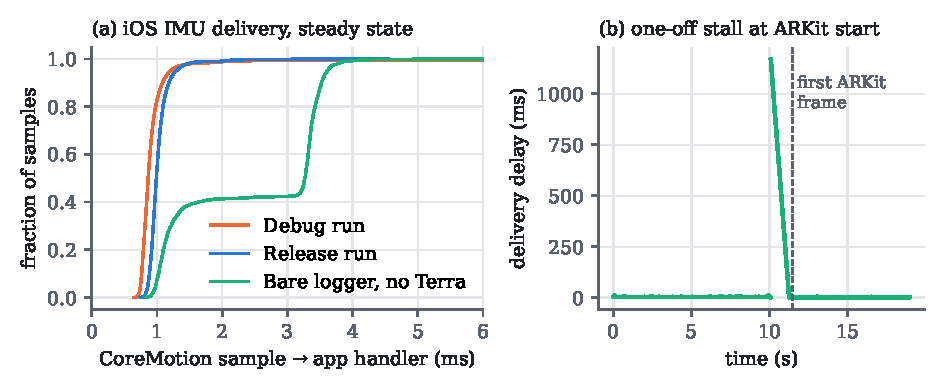
\includegraphics[width=0.95\textwidth]{figures/phone_timing_ios_delivery.pdf}
\caption{iOS IMU delivery, CoreMotion sample to app handler. (a) In steady state, delivery is under about 2~ms in the Debug and Release runs and under 5~ms for the bare logger with no Terra code running. (b) The one stall in the pilot: iOS held samples for 1.17~s while the ARKit session started.}
\label{fig:phone-timing-ios}
\end{figure}

\paragraph{iOS is not the cause.}
In every run iOS delivered IMU samples at 99--100~Hz, with p99 delivery between 2.0 and 2.3~ms (Figure~\ref{fig:phone-timing-ios}).
That leaves almost all of the 0.1~s budget to the app.
iOS stalled twice in all the data.
It held samples for 1.17~s while an ARKit session started, so the rover must not drive until tracking has run for a few seconds.
It also paused the IMU for 2.3~s at 311~s into the Debug run, with the phone in the \emph{serious} thermal state and AR frames also gapping up to 3.8~s.
The second stall's cause is unknown, and it is the main reason E6 must run for 90 minutes.

\begin{figure}[ht]
\centering
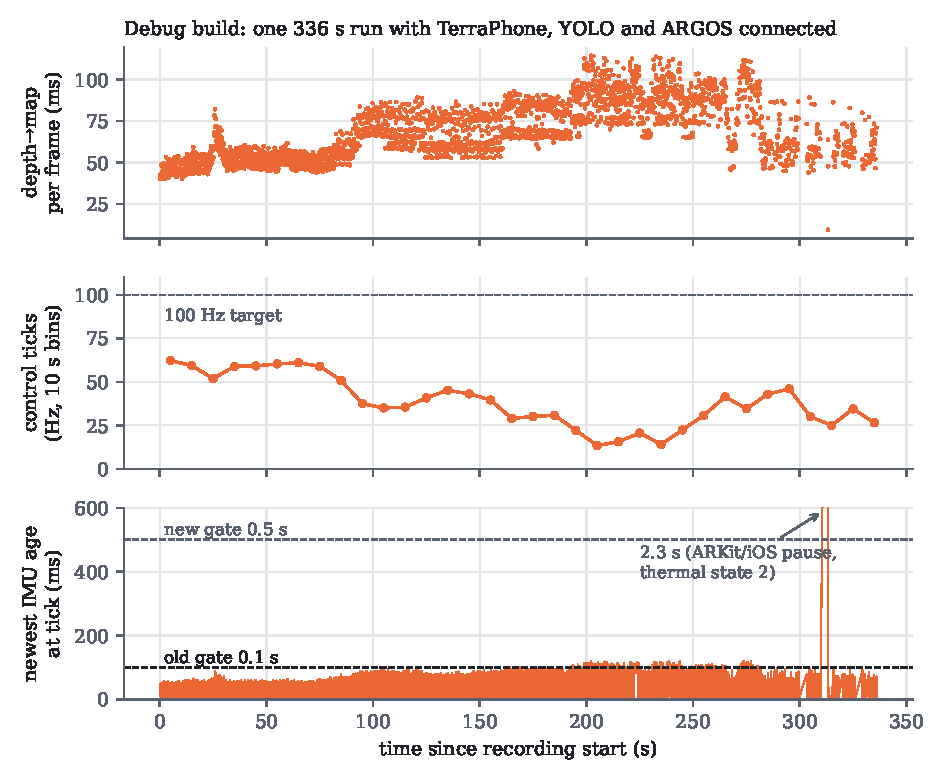
\includegraphics[width=0.85\textwidth]{figures/phone_timing_debug_timeline.pdf}
\caption{The Debug run (C2$^{*}$, 336~s). Top: time the Swift depth-to-map step held the control queue per depth frame. Middle: control ticks per second in 10~s bins. Bottom: age of the newest IMU sample at each tick, with the old 0.1~s gate and the 0.5~s gate of Terra PR~\#92.}
\label{fig:phone-timing-timeline}
\end{figure}

\paragraph{The Debug build is the cause.}
In the Debug build, all 233 stale ticks were attributed to Terra's control queue, and in each one the blocking task was the Swift depth-to-map step.
That step grew from about 45~ms per frame to over 100~ms during the run (Figure~\ref{fig:phone-timing-timeline}).
At 10~Hz it kept the queue 60\% busy, and the control loop ran at 39~Hz on average instead of 100.
The IMU samples reached the app within about 2~ms and then waited behind the map step.
In Release, the same step took 9--16~ms (p50) and never more than 30~ms, the queue was 7--12\% busy, and the loop ran at 96--100~Hz with no stale tick (Figure~\ref{fig:phone-timing-dvr}).
Release runs were done with the phone already hot, so heat alone does not explain the Debug slowdown.
The holds therefore came from unoptimised Swift on the control queue, not from iOS and not from the phone's hardware.
Field runs and every result in this thesis must use Release builds.

\begin{figure}[ht]
\centering
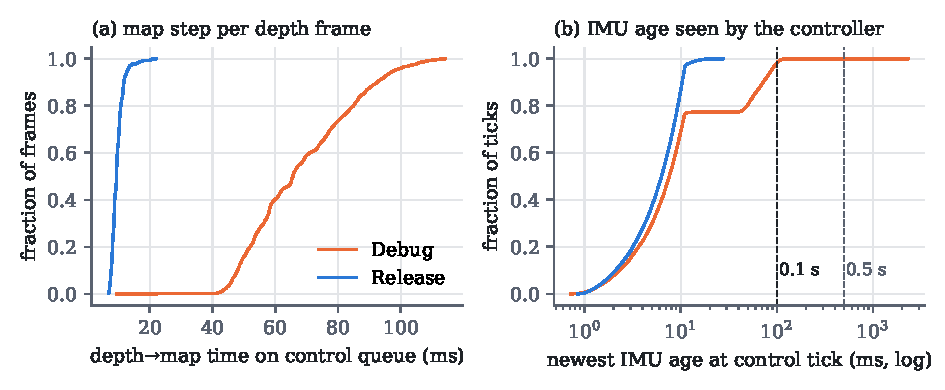
\includegraphics[width=0.95\textwidth]{figures/phone_timing_debug_vs_release.pdf}
\caption{Debug against Release, as empirical cumulative distributions. (a) Depth-to-map time per frame. (b) Age of the newest IMU sample at each control tick (log scale), with the 0.1~s and 0.5~s gates.}
\label{fig:phone-timing-dvr}
\end{figure}

Terra PR~\#92 raises the IMU freshness gate from 0.1 to 0.5~s.
With that gate the Debug run would have had one stale tick, the 2.3~s iOS pause, instead of 233.
A looser gate hides queue delays rather than removing them, so the Release numbers, not the gate, are the evidence for R5.

\paragraph{Caveats.}
The three Release runs total 212~s, and none is longer than the roughly 150~s the Debug slowdown took to appear.
All runs were static, and only one phone was tested.
\todo{Run C5 (driving) and a C2/C3 Release run of at least 10 minutes, and report whether the late iOS IMU and AR stalls reappear.}

\subsection{E3: LiDAR obstacle detection from the rover}
\label{sec:phone-e3}

\paragraph{Evidence so far.}
Three failure cases came from the rover, not from the literature.
A body axis about 16$^\circ$ off gravity tilted the ground plane through the floor and turned bare floor beyond about 2~m into obstacles (Section~\ref{sec:auto-ground}); a mount saved with the wrong roll put the map in its fallback horizon band and marked a ring of floor as obstacles (Section~\ref{sec:rover-mount}); and glass returns no depth and is mapped free (Section~\ref{sec:auto-glass}).
The first two are calibration faults that the floor veto and the mount procedure now address; the third is a property of the sensor.
None of them gives the accuracy that R6 asks for.

\paragraph{Protocol (pending).}
The rover is parked with the phone at its 0.23~m mount height.
Targets are placed at 0.5, 1, 2, 3, 4 and 5~m along the camera axis and at $\pm 20^\circ$, positioned by tape or by OptiTrack markers.

\begin{center}
\small
\begin{tabularx}{\textwidth}{@{}l X@{}}
\toprule
Factor & Levels \\
\midrule
Target & 0.30~m box; 0.15~m tall block; chair (thin legs); 5-gallon bucket; standing person; glass door \\
Light & Indoor lit; mocap strobes on; outdoor overcast; outdoor noon sun on turf \\
Motion & Parked; driving toward the target at 0.3~m/s \\
Repeats & 3 captures per cell, each one \emph{Capture 3D} point cloud plus 10~s of map \\
\bottomrule
\end{tabularx}
\end{center}

Metrics: range error of the LiDAR returns on the target (mean and s.d.); whether the target's cell is occupied in the published map; the farthest distance at which each target is mapped; and, on 2~m~$\times$~2~m of bare floor with no target, false occupied cells per minute.
R6 passes if the 0.30~m box and the 0.15~m block are mapped at 3~m in every light condition, the range error is below 0.1~m, and the bare floor stays free.
\todo{Run E3; add a plot of mapped range against true range per light condition.}

\subsection{E4: On-phone object detection}
\label{sec:phone-e4}

\paragraph{Accuracy in simulation (done).}
Terra's YOLO bucket-and-ball model (\texttt{yolo26n-rover}, 640~px input, the same weights as the phone's Core ML package) was run at confidence 0.25 on frames from four parked rovers on the simulated NEXT field, with ground truth projected from the known layout and checked for occlusion with depth.
Table~\ref{tab:phone-e4} gives the result for buckets within 10~m; beyond 10~m, 1 of 126 buckets was found.

\begin{table}[ht]
\centering
\caption{E4 simulator results: buckets found within 10~m, October 27, 2026 (Zorvane).}
\label{tab:phone-e4}
\small
\begin{tabular}{@{}l r r r r r@{}}
\toprule
Run & Blue, ground & Blue, stand & Orange, ground & Orange, stand & False \\
\midrule
Noon, 256$\times$192 camera & 21/22 & 0/4 & 4/18 & 0/6 & 0 \\
Noon, 1024$\times$768 & 21/22 & 1/4 & 5/18 & 0/6 & 0 \\
Overcast, 1024$\times$768 & 8/18 & 1/3 & 14/14 & 1/4 & 2 \\
\bottomrule
\end{tabular}
\end{table}

Colour was always right when a bucket was found.
Recall depended on which side of the bucket was in shade, not on its colour: at noon the rovers facing the shaded side missed most orange buckets, and overcast light reversed which colour was missed.
Buckets on 1~m stands were mostly missed (3 of 17).
The median confidence of found buckets was about 0.75, below the 0.8 that L4 target search requires to confirm a target, so many true sightings would not count.
In simulation the model fails R7 for shaded and raised buckets, and the confirm threshold and the detector disagree.

\paragraph{Rate and accuracy on the phone (pending).}
Two gaps remain: how fast the detector runs on the phone while everything else does, and whether the simulator's accuracy transfers to real buckets.
The rate comes from the detector rows of E2's C3--C5 files: frames per second, and inference latency $t_{\text{done}} - t_{\text{sensor}}$ (p50, p99).
The first run with Terra's load, C2$^{*}$ in a Debug build, gave 4.5~Hz and 108 / 172~ms (p50 / p99). In Release the end-to-end latency fell to 71 / 80~ms at 4.3~Hz, and stayed under 100~ms (p99) with FPV on (Table~\ref{tab:phone-release}).
The field test places real ground and raised buckets of both colours at 2, 4, 6, 8, 10 and 12~m, in sun and shade, with the rover parked and then approaching at 0.3~m/s, 30~s per placement.
Metrics: recall and precision per distance, colour and height; the confidence distribution against 0.8; and the error of the reported bucket position against tape.
\todo{Fill the detector rate from E2 and run the field test.}

\subsection{E5: GNSS and compass on the rover}
\label{sec:phone-e5}

\paragraph{Evidence so far.}
Mounted near the drive motors, the compass read headings 30--50$^\circ$ off, which is why Terra fuses VIO yaw, GPS course and the compass (Section~\ref{sec:auto-outdoor}).
GPS accuracy on the rover has not been measured.

\paragraph{Protocol (pending).}
\emph{Static:} the rover is parked for 10~minutes on each of four points with known coordinates on the field (from an RTK receiver if one is available; otherwise the corners of a taped 20~$\times$~10~m rectangle, which gives relative error only).
\emph{Driving:} 30~m straight runs at 0.3 and 0.5~m/s, five each way.
\emph{Compass:} the phone at its normal mount and raised 0.2~m further from the motors, motors off and on.
Metrics: horizontal error CEP50 and CEP95; the fraction of fixes whose error is inside the reported horizontal accuracy; time to first good fix; GPS course error against VIO heading at each speed; compass error against the fused heading per mount and motor state.
R8 passes if CEP95 $\le$ 10~m on the open field.
\todo{Run E5 on Field 3 or a comparable open field.}

\subsection{E6: Endurance and thermal behaviour}
\label{sec:phone-e6}

\paragraph{Protocol (pending).}
One 90-minute run with the full stack on: tracking, LiDAR depth and mesh, mapping, the detector, FPV to ARGOS and GPS.
It is done twice, indoors on the bench with the wheels off the ground, and outdoors on the field in daylight, both starting from a full charge and a cool phone.
The sensor-timing probe records the iOS thermal state (nominal, fair, serious, critical), low-power mode, and battery level and charging state at the start and on every change (Terra PR~\#90).
Metrics, per minute: battery level; thermal state; detector frames per second; control-tick lateness p99; stale-IMU holds.
R9 passes if the phone never reaches \emph{critical}, has battery left at 90 minutes, and the detector rate and tick lateness at the end are within 20\% of the first ten minutes.
\todo{Run E6 once Terra PR~\#90 is merged and built.}

\section{Verdict so far}
\label{sec:phone-verdict}

Table~\ref{tab:phone-verdict} collects the results.

\begin{table}[ht]
\centering
\caption{Is the iPhone suitable? Status of each requirement as of October 27, 2026.}
\label{tab:phone-verdict}
\small
\begin{tabularx}{\textwidth}{@{}l l X@{}}
\toprule
Requirement & Verdict & Basis \\
\midrule
R1 VIO scale & Fail as measured & 0.91 in the mocap room; E1b decides whether a fixed correction fixes it \\
R2 VIO noise & Pass & E1 \\
R3 VIO delay & Pass & E1 \\
R4 Heading (VIO) & Pass & E1; compass part pending in E5 \\
R5 IMU delivery & Pass in Release (static, $\le$122~s); fail in Debug & iOS delivery p99 $\le$ 2.3~ms in all runs; Release: 0 stale ticks in 212~s, IMU age max 37~ms; Debug: 233 stale ticks from the Swift depth-to-map step; iOS stalls of 1.17~s (ARKit start) and 2.3~s (late, hot); long and driving runs pending \\
R6 Depth & Pending & Failure cases known; accuracy from E3 \\
R7 Detection & Fail in simulation & Shaded and raised buckets; confidence below confirm threshold; real-world pending \\
R8 GNSS & Pending & E5 \\
R9 Endurance & Pending & E6; early sign: serious thermal state after about 4~min in C2$^{*}$ (rover still, Debug) \\
\bottomrule
\end{tabularx}
\end{table}

The evidence so far supports a qualified version of the thesis claim.
The parts of the phone that the inner control loop depends on most, VIO noise and delay, VIO heading and iOS's IMU delivery, meet their requirements with margin.
The failures are of different kinds.
The stale-IMU holds came from the Debug build of Terra's own Swift map step on the control queue, and disappeared in Release (Figure~\ref{fig:phone-timing-dvr}); what remains open is whether iOS stays clean over a long, driving run.
The VIO scale error is small enough that the loop stays stable and the rover stays consistent with its own map (Section~\ref{sec:auto-state-validation}); it matters for absolute distances, and the literature both reports similar errors~\citep{feigl2020localization} and predicts them for ground vehicles~\citep{wu2017vinswheels}.
The detector's failures are failures of a model trained for this task, not of the phone's hardware.
What remains open is the claim's hardest part: whether all of this holds with every subsystem running at once, on turf, for 90 minutes.
E2, E4 and E6 test that directly.
